\graphicspath{{chapters/TumorEvAndVesciclesImages/}}

\chapter{Extracellular vescicles}

\section{Introduction to EVs}

  "Extracellular vesicles are \textbf{membrane-enclosed nanoscale particles} released from essentially all prokaryotic and eukaryotic cells that \textbf{carry proteins, lipids, RNA and DNA}." (\textit{"RNA delivery by extracellular vesicles in mammalian cells and its applications", O’Brien et al, 2020 - Nature Reviews Molecular Cell Biology}). The content of an extracellular vesicle (EV), including membrane proteins, is usually referred to as \textbf{cargo}.

  EVs present many different surface proteins, mainly \textbf{tetraspanins} (commonly used markers to identify them) but also receptors, adhesion molecules and immune system ligands; these molecules are responsible of the targetting function, meaning that they define which cells the EV should interact with. 

  \begin{figure}[H]
  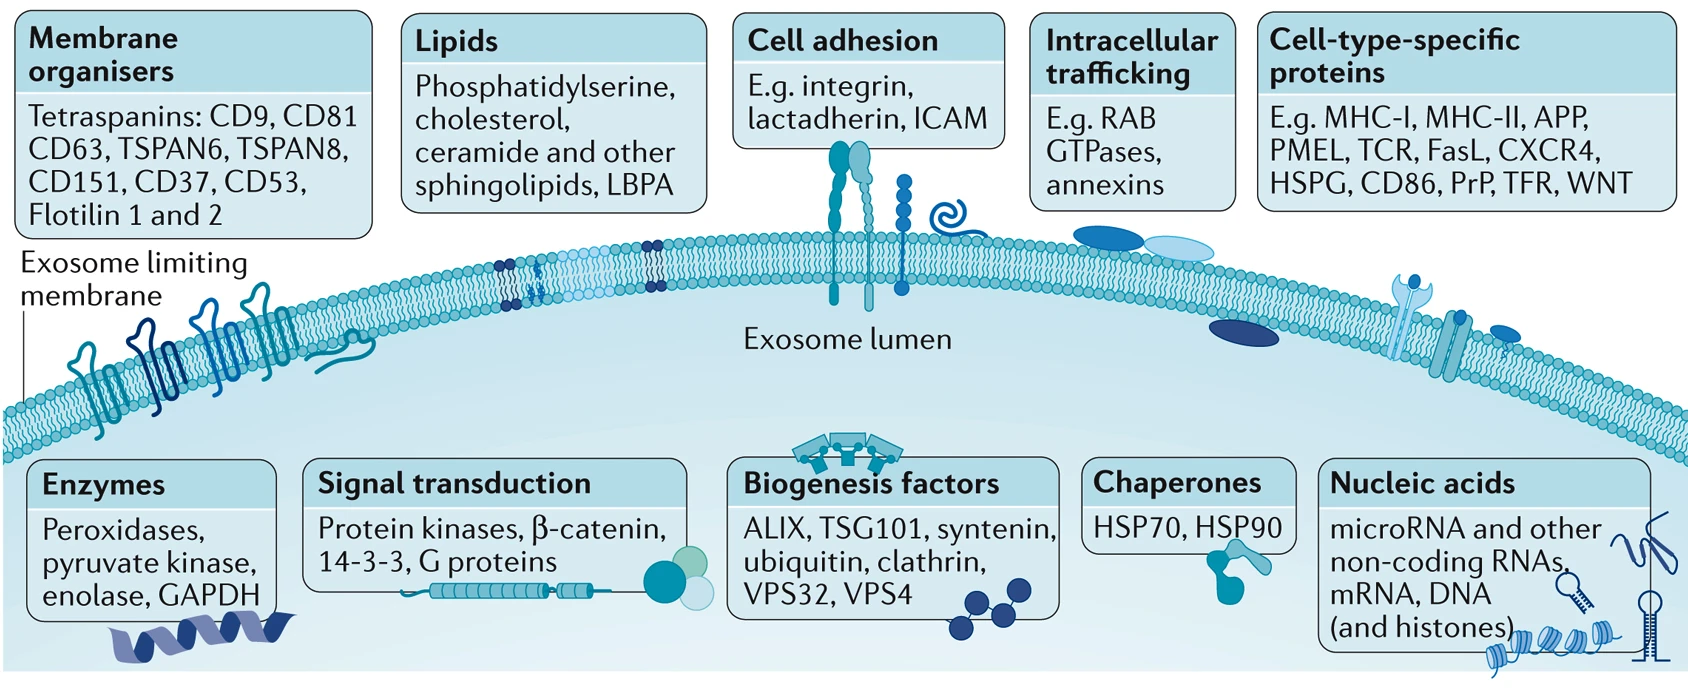
\includegraphics[scale=0.34]{image_07.png}
  \end{figure}
   
  The cargo of an EV tends to reflect the state of the cell that produced it; this way EVs become a way to transport material from a cell to another, but mostly to comunicate even at long distances (since EVs can enter the blood stream).

  Different types of EVs exist (different cargo, dimensions, genesis...). In older literature EVs were calssified based on the cells that produced them and/or their size and/or function (e.g. large oncosomes); now the International Society for Extracellular Vesicles (ISEV) suggests to classify EVs into three categories, \textbf{exosomes}, \textbf{microvesicles} and \textbf{apoptotic bodies}. The respective characteristics are summarized in the following table.
  
  \begin{figure}[H]
  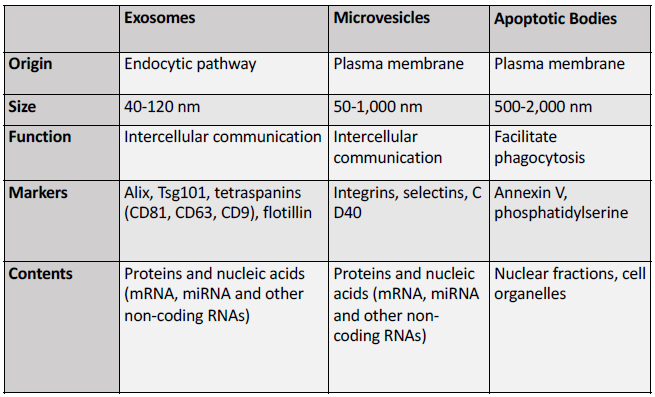
\includegraphics[scale=0.8]{image_05.png}
  \end{figure}

  Notice that size is not enough to subdivide them since there are overlaps. A way better way of classifying EVs is by their genesis:
  \begin{itemize}
    \item Exosomes originate from \textbf{multivesicular bodies}. Multivesicular bodies are organelles whose membrane buds inward creating \textbf{intraluminal vesicles}; then when the multivesicular bodies merge with the plasmatic membrane their content is released into the extracellular environment and intraluminal vesicles become exosomes.
    \item Microvesicles originate from outward budding of the plasmatic membrane.
    \item Apoptotic bodies are generated from apoptotic cells through various mechanisms.
  \end{itemize}

  \begin{figure}[H]
  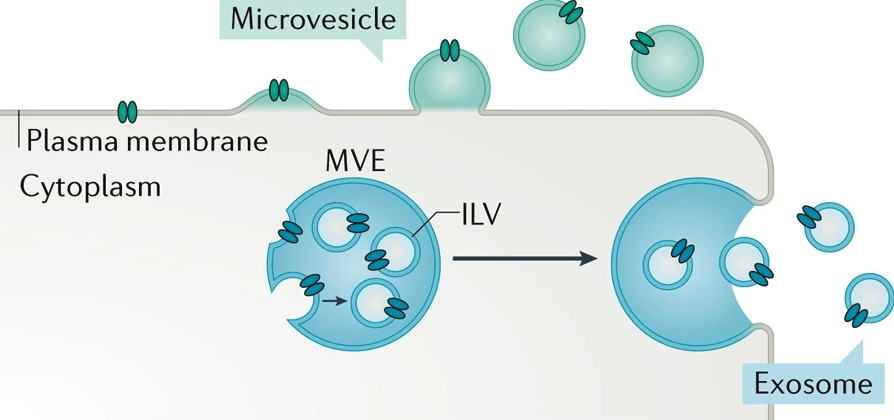
\includegraphics[scale=0.5]{image_06.png}
  \end{figure}

  The EV genesis defines the cargo and the surface markers, which define the target cell for the EV. Surface markers can be used in \textbf{flow cytometry} to divide these three populations. It is important to note that the content of exosomes and microvesicles is not just a portion of the cytoplasm of the cell generating them, but it is also enriched in specific molecules thanks to \textbf{selective sorting} mechanisms (only some of which are known), especially for proteins and RNAs.

  EV uptake by target cells can occur through different modalities (depending on target cell, vesicle size and others):
  \begin{itemize}
    \item Phagoytosis 
    \item Macropinocytosis 
    \item Clatrhrin dependent endocytosis
    \item Receptor mediated endocytosis 
    \item Fusion with the plasmatic membrane
  \end{itemize}


\section{Medical applications of EVs}

  Due to the aforementioned facts that:
  \begin{itemize}
    \item Almost all cells produce EVs, cancer and other diseased cells included
    \item The cargo reflects the functional status of the secerning cell
    \item EVs can convey signal through long distances
  \end{itemize}
  EVs are being studied more and more for clinical applications, mainly to understand disease pathogenesis (and eventually how to act on it) and to potentially use them in early-screening assays. 
  The fact that tumor derived EVs play a major role in reorganizing the surrounding environment has already been proven: tumor derived EVs induce endothelial proliferation and thus neoangiogenesis, fibroblast differentiation and extracellular matrix remodeling. This last aspect is especially relevant since EVs can create niches that facilitate the metastatic process. 

  One other significant advantage of EVs is the fact that they can be obtained through liquid biopsy, together with circulating tumor cells (CTCs), cell free DNA (cfDNA) and ribolipoproteins. Liquid biopsy generally refers to blood samples, therefore a non invasive technique to study the disease.
  Integrating transcriptomic data from EVs with other techniques could provide efficient biomarkers for early detection and biomarkers to easily measure overtime to track tumor evolution or response to a treatment. 

  In order to use EVs in clinical applications, a consistent and reproducible way of extracting EVs from the liquid biopsy is needed. In the context of the PRIME project (PRostate cancer plasma Integrative Multi-modal Evaluation consortium), different methods to extract EVs from plasma (from prostate cancer and healty patients) have been tested and compared, those methods being:
  \begin{itemize}
    \item \textbf{Nickel-based isolation (NBI)}, which utilizes the fact that EVs are negatively charged, hence they are attracted by positively charged nickel beads; the beads are then retrieved using magnets and the EVs are eluted from their surface. 
    \item \textbf{Size exclusion cromatography (SEC)}, which is a chromatographic technique in which the retention time of an object in the column depends on their size (the bigger the object, the fewer the pores of the stationary phase it can enter into, the faster the object is eluted). This technique requires knowing the elution times of the EVs, which can be difficult considering their high heterogeneity.
    \item \textbf{Ultracentrifugation (UCFG)}, meaning centrifugation at around 22000 RPM for some hours. EVs are too small to sediment using regular benchtop centrifuges. 
  \end{itemize}
  The total amount of RNA obtained from each extraction was measured using SMARTseq kit. 

  The result was that different isolation methods were highly reproducible on homogeneous samples (EVs from prostate cancer cell lines culture medium), while the different methods showed higher variability on heterogeneous samples (EVs from blood). This shows that different isolation methods isolate better different EV populations, expecially in samples such as blood which contains a miriad of EVs with different origin and characteristics, since all healty tissues produce EVs that mix with tumor derived ones in the blood. This leads to the need to identify which method is the best in order to enrich tumor derived EVs rather than healthy tissue derived ones; no standard protocol for the isolation of EVs and the analysis of their transcriptome is available. 
  
  Another challenge, deriving from the use of EVs, is the fact that RNA signal deriving from multiple populations is difficult to interpret. Ideally one would need some way to deconvolute the signal into the components associated with each cell population; in order to do so, two potential approaches are possible: 
  \begin{itemize}
    \item \textbf{Supervised deconvolution}, which means using known cell line signatures to split the signal and compute the fraction of contribution for each population (one tool that does this is CIBERSORT). The main problem with this method is that it is not possible to get the signal for unknown cell populations; moreover it is difficult to define cell population specific signatures since we do not have pure EVs populations obtained from blood. 
    \item \textbf{Unsupervised deconvolution}, which means using unsupervised clustering algorithms to subdivide the signals into populations; the problem is that these approaches tend to be less sensitive and the identification of the clusters is not simple. Still, this allows to identify not previously known cell populations.
  \end{itemize}
  Deconvolution approaches are therefore plausible but not well established.

\section{EVs conference}
  Notes from the conference \textit{"Extracellular vesicles as diagnostic and therapeutic tools for kidney diseases, Benedetta Bussolati, Dept. of Molecular Biotechnology and Health Sciences, University of Torino, 12 May 2022"}.

  \textit{DISCLAIMER}: they might not be perfect but they should suffice for a general idea of the concept
  
  EVs are part of the secretome produced by stem cells in order to try and induce tissue regeneration after damage, since they do not act directly in the regeneration process by differentiating. For this reason stem cell derived EVs (scdEVs), are subject of study for potential tissue therapies. Most studies have been performed on mesenchymal stem cell derived EVs, but some studies have shown that, despite the great heterogeneity of EVs produced by stem cells, little to no difference was found between mesenchymal stem cells derived EVs and other scdEVs. Of this heterogeneous population (especially regarding the expressed tetraspanins), small EVs seem to be the ones which are more associated to tissue regeneration; moreover small EVs are the safer ones for potential medical applications since they do not display HLA or tissue factor, that are sometimes present in bigger vesicles and that could lead to immune response and coagulation respectively. A very big spectrum of genes is regulated simultaneously through EVs; to support the role of EV content in the regenerative process, DROSHA KO models (which have impaired miRNA loading into EVs) lose most of their therapeutic effect.

  One way to analyse EVs is MACSPlex, a cytofluorimetric tool with beads and detection antibodies for tetraspanins; that being said, especially for medical purposes, better and more standardized ways to quantify, identify and test the potency of EVs are still needed. Notice that the potency of an EV, meaning its ability to induce a certain response, is highly application dependent. 

  Regarding the activity of EVs on kidney diseases, there have been different studies:
  \begin{itemize}
    \item Renal damage markers in kidney injury model decrease overtime in presence of stem cells or just scdEVs; the responses in the two cases are basically the same, suggesting that most of the therapeutic effect of stem cells in kidney diseases is due to EVs.
    \item Repeated administrations of scdEVs to diabetic nephropaty models reduce inflammation and fibrosis
    \item In healhy patients most vesicles reach liver and spleen, while in diseased patients one can find more EVs than usual in the damaged site; this supports both a specific and an aspecific targetting of EVs to the damaged area. This holds true even in kidney disease models, where administered intravenous EVs reach the kidneys within 15 minutes. 
    \item A phase 1 study has been conducted on the use of scdEVs in kidney diseases. 
    \item Urine derived EVs are comparable in potency with MSCs EVs. Urine derived EVs are all generated from kidney cells, since no EVs from the blood stream can pass the glomerular filtration membrane; this also means that urine derived EVs could be used as a diagnostic tool for kidney diseases. 
    \item Klotho, a recently discovered hormone, is produced mostly by the kidney both in a transmembrane and in a soluble form. Klotho KO murine models have a significantly shorter lifespan and a faster aging process. Klotho can be found both in urine and blood. Moreover klotho has been found coexpressed with tetraspanins, confirming its presence EVs. By providing recombinant klotho EVs to a klotho KO mouse model, the healthy phenotype is rescued; moreover providing klotho through EVs rather than by direct injection is more efficient. 
    \item Autologous urinary EVs seem to have a beneficial effect in kidney injury model.
    \item CD133+ is a marker for regenerative kidney cells in adult humans; studies have tried to test if its expression on urinary EVs correlates with the outcome of kidney transplant. Healthy human urinary EVs display very high levels of CD133+. Bad responders to kidney transplant displayed lower levels of CD133+ compared to good responders, but both had significantly lower levels of expression compared to healthy individuals. Blood and urine samples of kidney transplant patients were collected at various timepoints during a period of one year. Samples were centrifuged to remove bigger debris, analyzed using MACSPlex and then normalized for the number of identified tetraspanins. Some of the patients did not recover while others did; by analyzing samples from 10 days after the transplant was possible to predict which patients would recover and which would not. Both in blood and urine EVs were found different biomarkers (among which CD133+) whose concentration was significantly higher in individuals that would recover. 
  \end{itemize}

